\chapter{Aufnahme von Koordinatenpunkte}
\section{Problem}
Wenn ein Koordinatenpunkt aufgenommen werden will, gibt es mehrere Probleme auf die man stößt. 

Zum einen kann nicht gleichzeitig die x- und y-Komponente bestimmen werden, dies muss nacheinander folgen. 
Grund hierfür ist dem Aufbau des Touchscreens geschuldet.

Bei der Inbetriebnahme ergibt sich ein weiteres Problem ergeben. Falls der Touchscreen nicht betätigt wird, gibt der Mikrocontroller trotzdem Werte aus. 
Dabei handelt es sich um Werte die keinen Sinn ergeben und die Steuerung der Maus z.B. bei einer Ruhephase stören würden.

Bei einer Messreihe kann es vereinzelt zu einem Wertesprung kommen. 
Dieses Problem ist der Messunsicherheit des Systems geschuldet. Diese Sprünge gilt es aus der Messreihe heraus zu filter und zu glätten.

\section{Lösungsansatz}
Bevor Werte ausgegeben werden, wird geprüft ob das der Touchscreen betätigt wird. Ist dies der Fall so soll die Messung durchgeführt werden.

Um eine Koordinatenkomponente zu bestimmen, benötigt man drei Anschlüsse des Touchscreens. Zwei davon sind in der Richtung die man messen möchte und der dritte Anschluss ist einer der beiden übrigen Anschlüsse. 
Mit diesem wird der Spannungsteiler auf gespannt um den Wert der Koordinate zu bestimmen.
In den Abbildungen \ref{fig:xylesen} auf Seite \pageref{fig:xylesen} wird dieser Lösungsansatz veranschaulicht. 

Bei dem Lesen der x-Komponente \figref{fig:xlesen} wird der Pin \verb$X_Le$ (steht für X-Links) auf eine Spannung von \SI{5}{V} gesetzt. Der Pin \verb$X_Ri$ (steht für X-Rechts) wird auf \SI{0}{V} gezogen.
Der Pin  \verb$Y_Up$ (steht für Y-Oben) wird auf den Modus \verb$Hi Z$ (Hohe Impedanz) gesetzt. Mit einer hohen Impedanz auf  \verb$Y_Up$ kann der Widerstand \verb$R_yup$ vernachlässigt werden. 
Um die y-Komponente zu lesen werden die Anschlüsse wie in Abbildung \ref{fig:ylesen} auf Seite \pageref{fig:ylesen} gesetzt. Der Pin \verb$Y_Up$ auf \SI{5}{V} und der Pin \verb$Y_Lo$ (steht für Y-Unten) auf \SI{0}{V} gesetzt. 
Der Pin \verb$X_Le$ wird auf den Modus \verb$Hi Z$ gesetzt. 

Die Pins die bei der Messung nicht miteinbezogen sind, werden in den jeweiligen Schaltungen deaktiviert. 

Um nun noch eine Messunsicherheiten aus zu filtern sollen, bei der Messung einer Koordinatenkomponente, mehrere Messpunkte aufgenommen werden. 
Diese werden anschließend über ein Filter-Funktion ausgewertet. Der Wert der bei der Auswertung als Ergebnis herauskommt, wird als gemessene Koordinatenkomponente ausgegeben.
Das Schaltbild hier zu ist in Abbildung \ref{fig:schaltbild} zu sehen. 

\begin{figure}[ht!]
    \begin{subfigure}{0.49\textwidth}
        \centering
        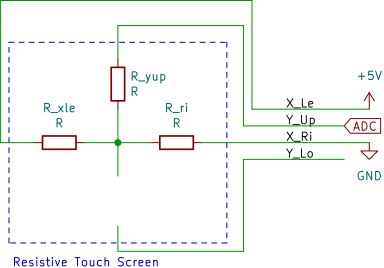
\includegraphics[width=\textwidth]{fig/xlesen.png}
        \caption{in x-Richtung}
        \label{fig:xlesen}
    \end{subfigure}
    \hfill
    \begin{subfigure}{0.49\textwidth}
        \centering
        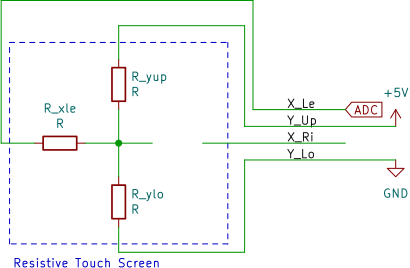
\includegraphics[width=\textwidth]{fig/ylesen.png}
        \caption{in y-Richtung}
        \label{fig:ylesen}
    \end{subfigure}
    \caption{Schaltbild für das Messen der Koordinatenpunkte}
    \label{fig:xylesen}
\end{figure}
\begin{figure}[ht!]
    \centering
    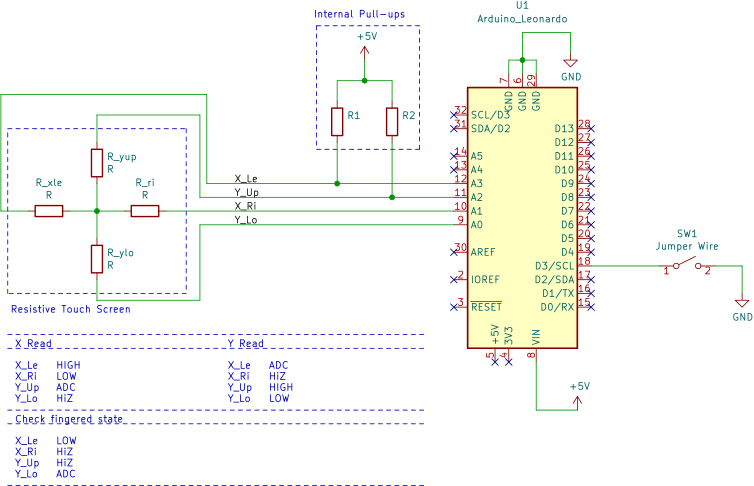
\includegraphics[width=\linewidth]{fig/schaltbild.png}
    \caption{Schaltbild des Projekts}
    \label{fig:schaltbild}
\end{figure}
Die einzelne Lösungsansätze werden in der Arduino-Umgebung umgesetzt. Der Programmablauf ist in der Abbildung \ref{fig:flowchart} auf der Seite \pageref{fig:flowchart} als Flow-Chart dargestellt.

\begin{figure}
    \centering
    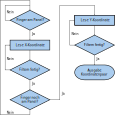
\includegraphics[scale=0.45]{fig/flow_chart.png}
    \caption{Darstellung des Programmablaufs}
    \label{fig:flowchart}
\end{figure}
\section{Umsetzung des Lösungsansatz}
\section{Filterung der Messpunkte}